\documentclass[12pt]{article}
\usepackage{hyperref}
\usepackage{graphicx}
\usepackage{float}

\title{ECRYP Project - Sieve of Eratosthenes}
\author{Krzysztof Rudnicki 307585 \\ Bartłomiej Dybcio 303854}

\begin{document}
\maketitle
\section{Description of the used algorithm}
Sieve of Eratosthenes is used to find all prime numbers below certain limit Lets call this limit $n$ \\ 
It starts with number 2, which is the first prime number and marks all multiplies of this number (up to predefined limit) as composite (not prime), those numbers will be later ignored \\ 
Then it takes next available number (3) and does the same thing \\ 
This is repeated until there are no more numbers below the limit which are neither prime nor crossed out \\ 
Then we return the list of all non-crossed out (prime) numbers \\ 
We used more optimized version of this algorithm and cross out composites only up to $\sqrt{n}$ in the main loop \\ 
\begin{figure}[H]
    \caption{Sieve of erastosthenes example for numbers up to 120, prime numbers on the right, darker colors show prime numbers, lighter colors show numbers which were checked while checking whether given number was prime \href{https://en.wikipedia.org/wiki/Sieve_of_Eratosthenes}{SOURCE} }
\centering
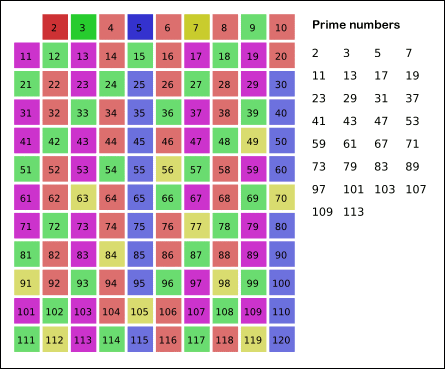
\includegraphics{screenshoot/algorithm_description.png}
\end{figure}
\section{Functional description of the application}
First we define the limit, we name this limit as $num$ which will decide how many numbers we will check, either by user interface or we hard code it in \\ 
We define boolean list which will be used to distinguish between prime and composite numbers \\ 
We start with number 2 and assign it to variable named $p$ \\ 
Then we calculate the primes using Sieve of Eratosthenes using nested while loops \\ 
External loop goes through numbers smaller than $\sqrt(num)$, starting with current value of $p$ \\ 
It checks if the number we are currently was checked out by checking the value of boolean table \\ 
if it was not checked out it gets a new number which is the $p$ multiplied by 2, then it goes into inner loop \\ 
inner loop sets all multiplicities of $p$ as crossed out by setting their value in boolean table to false \\ 
then we increment the $p$ and the whole loop repeats until we run out of numbers \\ 
we return array of prime numbers to function which prints those numbers 

\begin{figure}[H]
    \caption{Example of full program use }
\centering
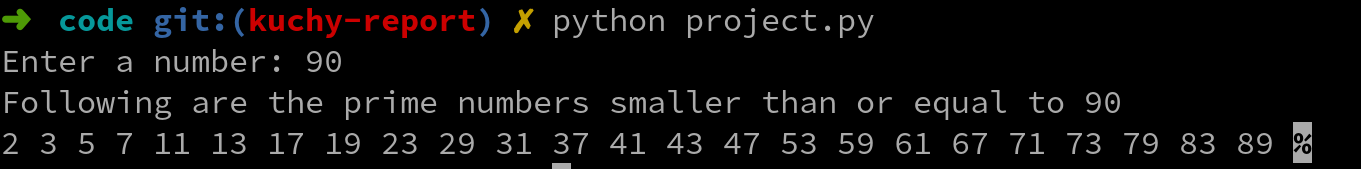
\includegraphics[width=\textwidth]
{screenshoot/program_use.png}
\end{figure}

\subsection{Input data format}
There is single input, variable named $num$ which is the upper limit of numbers to checked \\ 
It is a simple int variable, it cannot be less than 2 and has to be a whole number. 
\subsection{Output text on console}
As an output we put out all input prompts which ask for an upper limit, and the list of prime numbers found by our algorithm. 
\subsection{Format of output data}
Output data is a string
\subsection{Description of designed code structure}
There are three code blocks, sieve\_of\_eratosthenes, print\_sieve and main function executed at the beginning, main functions gets no arguments and outputs string consisting of prime numbers, print\_sieve function receives number which describes how many numbers should be checked in the sieve, similarly sieve\_of\_erastosthenes takes this number as an argument, and returns list of all prime numbers found by the sieve.

\begin{figure}[H]
    \caption{Flowchart of code flow }
\centering
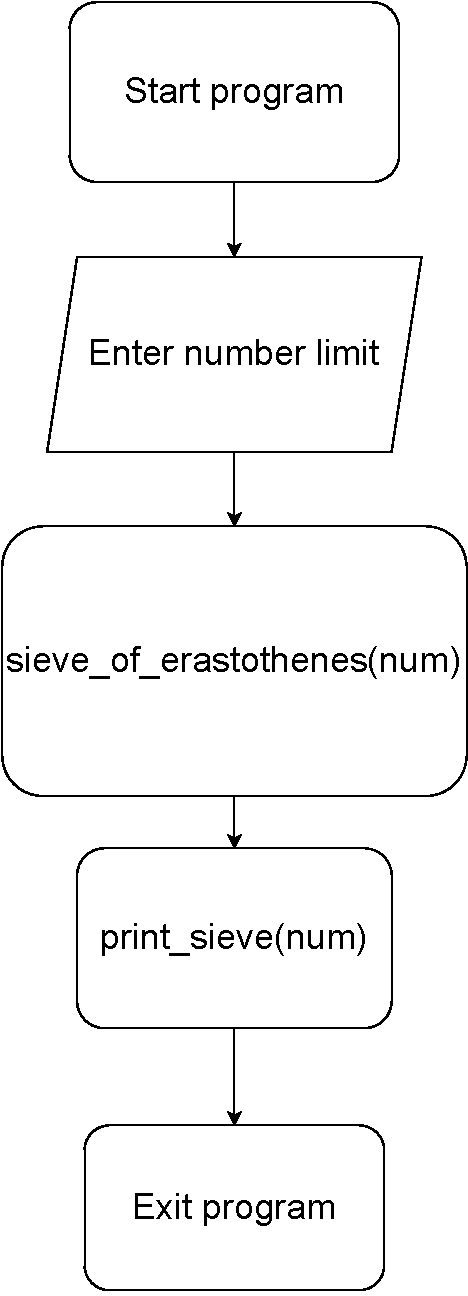
\includegraphics[height=\textwidth]
{screenshoot/code_structure.pdf}
\end{figure}



\section{Tests}
We did three types of tests, positive tests which inputted prime numbers into the sieve and checked if the sieve correctly validated them as prime, negative tests which inputted composite numbers into the sieve and checked if the sieve correctly determined them to not be prime. \\ 
We know which numbers are prime and which are composite based on the reference value which source was given below. 
\subsection{Source of reference values}
All reference values were taken from: \href{http://www.naturalnumbers.org/primes.html}{http://www.naturalnumbers.org/primes.html}

\subsection{Correctness of results}
All of the tests passed successfully with upper limit as high as 10000

\begin{figure}[H]
    \caption{Test results for prime numbers}
\centering
\includegraphics[width=\textwidth]
{screenshoot/prime_tests.png}
\end{figure}

\begin{figure}[H]
    \caption{Test results for composite numbers}
\centering
\includegraphics[width=\textwidth]
{screenshoot/composite_tests.png}
\end{figure}



\end{document}